\part{Learning Systems}

%\usepackage{natbib}
\usepackage{graphicx,color}
\usepackage{amsmath, amssymb}
\usepackage{listings}
\usepackage{algorithm2e}
%\usepackage{paralist}
\usepackage{hyperref}
\usepackage{tcolorbox}
\usepackage{diagbox}
\usepackage{algorithm2e}
\usepackage{tikz}
\usepackage{listings}

\renewcommand{\lstlistingname}{Algorithm}
\newcommand{\bdw}{\mathbf{\Delta w}}
\newcommand{\bSig}{\pmb{\Sigma}}
\newcommand{\bmu}{\pmb{\mu}}
\newcommand{\rT}{\mathrm{T}}
\newcommand{\bb}{\mathbf{b}}
\renewcommand{\bf}{\mathbf{f}}
\newcommand{\bm}{\mathbf{m}}
\newcommand{\bp}{\mathbf{p}}
\newcommand{\br}{\mathbf{r}}
\newcommand{\bs}{\mathbf{s}}
\newcommand{\bt}{\mathbf{t}}
\newcommand{\bx}{\mathbf{x}}
\newcommand{\by}{\mathbf{y}}
\newcommand{\bw}{\mathbf{w}}

\newcommand{\bbR}{\mathbb{R}}
\newcommand{\bbE}{\mathbb{E}}
\newcommand{\cL}{\mathcal{L}}
\newcommand{\cN}{\mathcal{N}}
\newcommand{\cD}{\mathcal{D}}
\newcommand{\cT}{\mathcal{T}}
\newcommand{\cE}{\mathcal{E}}
\newcommand{\cM}{\mathcal{M}}
\newcommand{\cV}{\mathcal{V}}
\newcommand{\cC}{\mathcal{C}}
\newcommand{\bA}{\mathbf{A}}
\newcommand{\bF}{\mathbf{F}}
\newcommand{\bI}{\mathbf{I}}
\newcommand{\bJ}{\mathbf{J}}
\newcommand{\bR}{\mathbf{R}}
\newcommand{\bS}{\mathbf{S}}
\newcommand{\bT}{\mathbf{T}}
\newcommand{\bX}{\mathbf{X}}
\newcommand{\lse}{\cL_\mathrm{LSE}}
\newcommand{\bPhi}{\mathbf{\Phi}}
\newcommand{\rd}{\mathrm{d}}
\newcommand{\inv}[1]{#1^{-1}}
\newcommand{\abs}[1]{\left\lvert #1\right\rvert}
\newcommand{\norm}[1]{\left\lvert\left\lvert #1\right\rvert\right\rvert}
\newcommand{\qmark}[1]{\mbox{}\hfill\textbf{[#1]}}
\newcommand{\argmin}{\operatorname*{arg\,min}}
\newcommand{\argmax}{\operatorname*{arg\,max}}
\newcommand{\var}{\operatorname*{var}}
\newcommand{\diag}{\operatorname*{diag}}
\newcommand{\tr}{\operatorname*{Tr}}
\newcommand{\dcos}{d_\mathrm{cos}}
\newcommand{\deuc}{d_\mathrm{euc}}
\newcommand{\figref}[1]{Figure~\ref{#1}}

%\newcommand{\figref}[1]{Figure \ref{#1}}
%\renewcommand{\eqref}[1]{Equation \eqref{#1}}
\tikzset{
  treenode/.style = {shape=rectangle, rounded corners,
                     draw, align=center,
                     top color=white, bottom color=blue!20},
  root/.style     = {treenode, font=\Large, bottom color=red!30},
  env/.style      = {treenode, font=\ttfamily\normalsize},
  dummy/.style    = {circle,draw}
}


\title{Introduction to Learning Systems}
\author{Amanda Cristina Fraga De Albuquerque\\
        Brendon Erick Euzebio Rus Peres\\
        Erikson Freitas de Morais\\
        Gilson Junior Soares\\
        Jose Lohame Capinga\\
        Marcella Scoczynski Ribeiro Martins}
\authorrunning{Supervised and Unsupervised Learning}

%\begin{document}
\maketitle

\section{Artificial Intelligence and Machine Learning}

In this part of the book we will provide an introduction to Artificial Intelligence and Machine Learning concepts;
In general, the term Artificial Intelligence (AI) refers to an area that has many strands and topics of study, where most are focused on making computers perform complex tasks, which were previously performed exclusively by humans.

Early AI studies tried and solved many problems that were considered difficult for humans but relatively easy for computers \cite{goodfellow2016}. These were problems that could be formally described using mathematical rules. As an example, we have the game of chess that, in 1997, champion Garry Kasparov lost to IBM Deep Blue (Figure \ref{fig:figure100}).

\begin{figure}
    \centering
    %\includegraphics[scale=0.1]{images/figure100.jpg}
    \includegraphics[scale=0.1]{"/Volumes/TOSHIBA EXT/Work/IEEE Activities/Education Portal 2021/book-git/IEEE-CIS-Open-Access-Book-Volume-1/Part 3 - Learning Systems/figure100.jpg"}
    \caption{IBM Deep Blue \cite{img:deepblue}.}
    \label{fig:figure100}
\end{figure}
\newpage

Over time, we began to realize that the difficulty did not reside in these problems, but in those that are easily, even instinctively and intuitively carried out by humans, such as recognizing familiar faces, understanding languages, etc. The point is that human beings, on a daily basis, receive and process huge amounts of information, so trying to make computers perform these activities only with rules described by us was not viable. Many, researchers started to develop techniques where the computer itself, through algorithms, learn to abstract these rules and information alone from raw databases, this is called Machine Learning.

Within the Machine Learning, we have a set of techniques and research areas and one of which uses a model based on biological brains, containing neurons and connections known as Neural Networks, often applied to several applications. In Figure  \ref{fig:figure101} we have a representation of neurons in the human cerebral cortex, where we can see the connections formed by them, which look like the neural network model in Figure \ref{fig:figure102}.

\begin{figure}
    \centering
%    \includegraphics[scale=0.30]{images/figure101.png}
    \includegraphics[scale=0.30]{"/Volumes/TOSHIBA EXT/Work/IEEE Activities/Education Portal 2021/book-git/IEEE-CIS-Open-Access-Book-Volume-1/Part 3 - Learning Systems/figure101.png"}
    \caption{Representation of the connection of neurons in the cerebral cortex \cite{cajal}.}
    \label{fig:figure101}
\end{figure}

Today, as we hear a lot about AI's, we tend to think this is a recent technique, but the idea of making computers mimic the brain's working scheme dates back to 1943, when Warren McCulloch and Walter Pitts suggested the idea in his article “A logical calculus of the ideas immanent in nervous activity” \cite{mcculloch1943}.

As can be seen in Figure \ref{fig:figure102}, neural networks are formed by layers, where the data enters through the Input layer, is processed in the Hidden layers and we have the output data in the Output layer. Each of these layers is formed by a number of neurons (in Figure \ref{fig:figure102} represented by circles) and their connections are represented by arrows.

\begin{figure}
    \centering
    %\includegraphics[scale=0.8]{images/figure102.png}
    \includegraphics[scale=0.8]{"/Volumes/TOSHIBA EXT/Work/IEEE Activities/Education Portal 2021/book-git/IEEE-CIS-Open-Access-Book-Volume-1/Part 3 - Learning Systems/figure102.png"}
    \caption{Artificial neural network.}
    \label{fig:figure102}
\end{figure}

In recent years, we have seen an ever-increasing range of applications for AI techniques. Our objective in this text is to introduce, mainly, the use of artificial neural networks in the area of computer vision, which is identified as one of the sub-areas of Artificial Intelligence as it seeks to reproduce some of the human capabilities from autonomous systems. The main interest of computer vision is to make computers perform functions similar to human vision, being able to receive visual data and with them perform recognition, classification and analysis. Analogous to the learning process of human beings, it is identified that the improvement in the performance of computer vision is strongly linked with the evolution of machine learning.

\section{Supervised and Insupervised learning}

Within machine learning algorithms, there is a feature that separates them into different types, based on their way of learning: supervised and unsupervised learning algorithms.

In supervised learning, algorithms previously have input-output pairs, that is, for each input we have prior knowledge of its output \cite{russell2016}, and from that, our algorithm must learn to generalize the entries well. We can formalize this as follows \cite{russell2016}:

Given a training set $\mathcal{T}$ of $\mathcal{N}$ pairs $(\mathbf{x}^{(1)},y^1),(\mathbf{x}^{(2)},y^2),\dots,(\mathbf{x}^{(N)},y^{(N)})$ where $\mathbf{x}^{(i)}$ are the input variables and $y^{(i)}=f(\mathbf{x}_{(i)})$ is the output variable, our algorithm must find the function $h$, known as a hypothesis, that best approximates $f$. To find out if our hypothesis approximates $f$ well, after having trained the algorithm, we use a set of tests - which contain different examples from the training set - and evaluate how well the algorithm generalizes (gives correct answers) to the new inputs.

In unsupervised learning, however, there is no response to the outputs of the algorithm, that is, it only receives input data. Therefore, one of the main tasks assigned to these types of algorithms is clustering, where the algorithm learns to find patterns in the input data and separate them into groups.


\bibliographystyle{unsrt}
\bibliography{bibliography}

%\end{document}
